


\subsection{Humoristes}
\begin{itemize}
\item Stéphane Guillon (le spectacle "En avant la Musique")
\item Fabrice Eboué
\end{itemize}

\subsection{Documentaires}
\begin{itemize}
\item Zétwal
\end{itemize}

\subsection{Court-métrages}
\href{http://www.dailymotion.com/video/xchpac_garde-fou_shortfilms}{Garde-fou (très original)}

\subsection{Sites internet}
\href{https://www.rottentomatoes.com/}{RottenTomatoes}: site US de critiques (compile les critiques de plusieurs sources)\\
\href{http://www.metacritic.com/}{Metacritic}: idem que RottenTomatoes. Valable aussi pour les séries télé et la musique\\
\href{http://www.telerama.fr/}{Télérama}: journal français de critiques\\
\href{http://iwdrm.tumblr.com/}{IWDRM}: des scènes cultes en .gif\\

\subsection{Films avec bonne BO}
\begin{itemize}
\item Le Lauréat: Simon \& Garfunkel
\item Ghost Dog: RZA \& The Wu Tang Clan
\item Drive: Kavinsky
\item Les films de Tarentino (Pulp Fiction...)
\item The Darjeeling Limited: musiques indiennes
\end{itemize}

\subsection{Jeux vidéo}
\href{http://www.jeuxvideo.com/jeux/playstation-3-ps3/00037095-classics-hd-ico-shadow-of-the-colossus.htm}{Shadow of the Colossus}: jeu très poétique. Voir aussi Ico, de la même équipe.\\
\href{http://www.jeuxvideo.com/jeux/playstation-3-ps3/00020227-portal.htm}{Portal}: jeu de réflexion\\
Metal Gear Solid 1, 2, 3 et 4: les classiques des jeux d'infiltration\\
Dead Space 1 et 2: survival-horror dans un univers inspiré d'Alien. Une vraie direction artistique pour les graphismes.\\
Demon's Souls et Dark Souls: RPG bien pensés sans baratin et pertes de temps inutiles.\\
Antichamber: jeu de réflexion assez philosophique.\\
Et aussi: Limbo, Flower...\\

\subsection{Littérature}
Cyrano de Bergerac, la pièce d'Edmond Rostand\\
Antigone, la pièce de Jean Anouilh\\
Balzac et la petite tailleuse chinoise (roman, Dai Sijie)\\
La grammaire est une chanson douce (roman, Erik Orsenna)\\

\subsection{BD}
Deathnote (manga): histoire très complexe et pourtant très cohérente. Et seulement 12 tomes, donc pas besoin de se ruiner.\\
Broussailles (les albums "Les baleines publiques" et "La nuit du chat"). Assez poétique.\\

%\newpage
%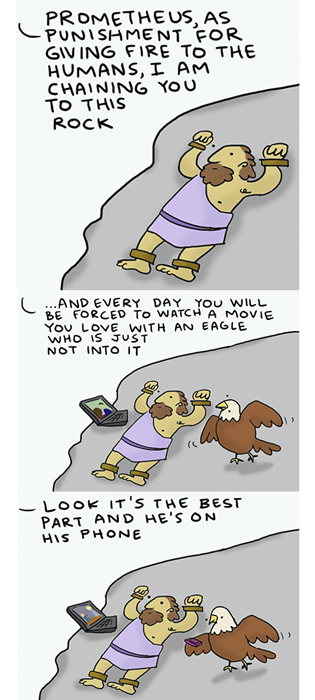
\includegraphics[width=0.70\textwidth]{humour/prometheus.png}

%\newpage
%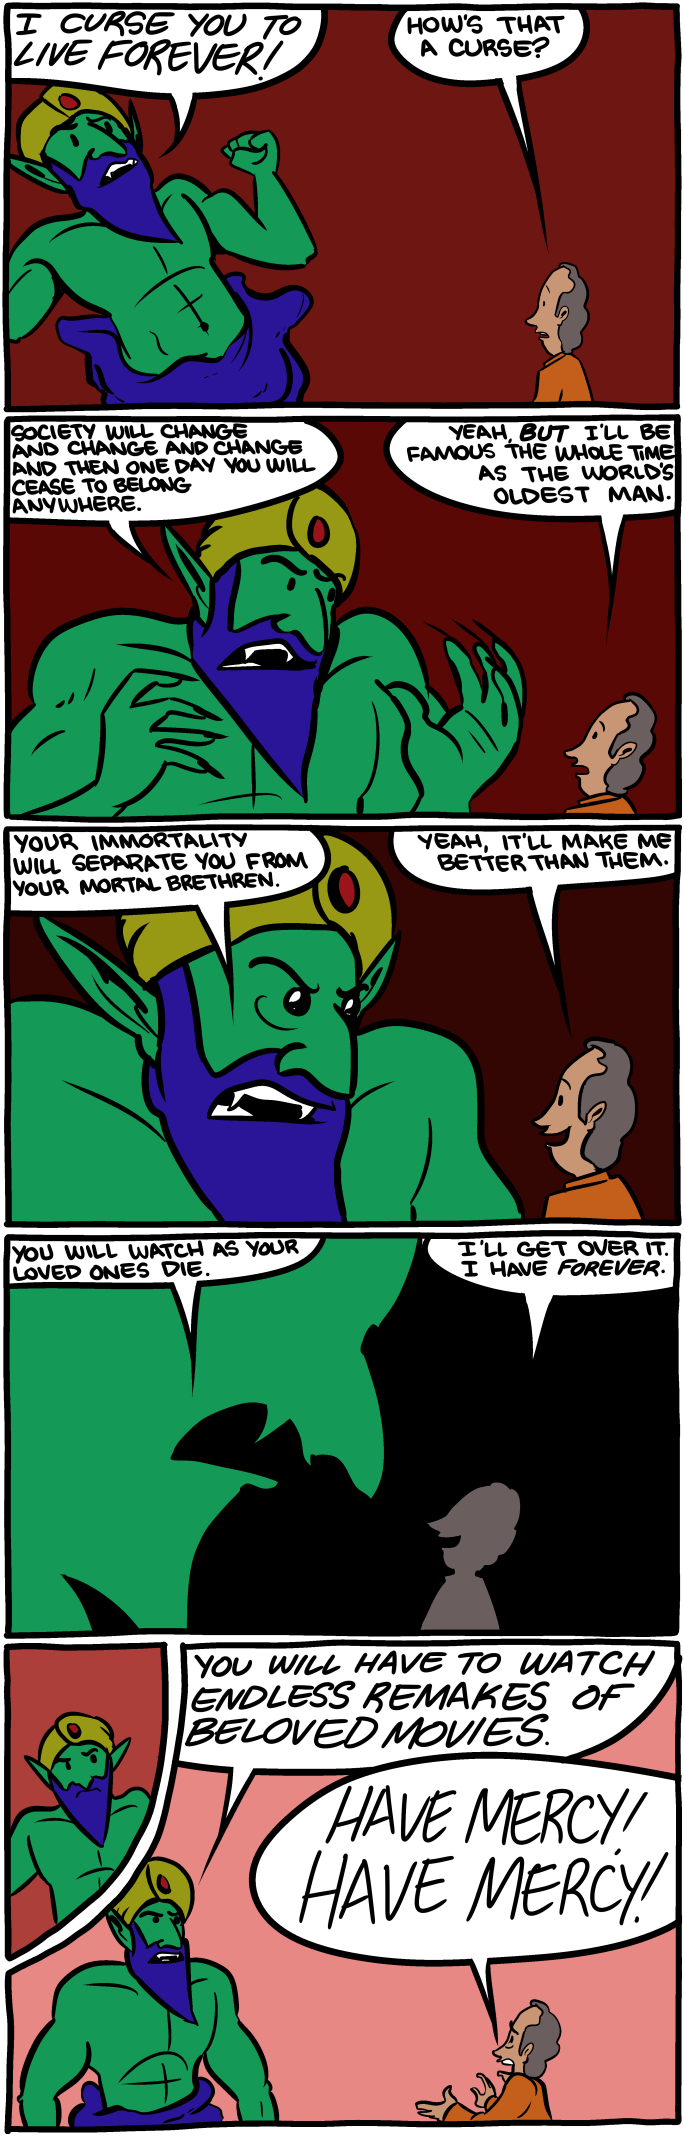
\includegraphics[width=0.50\textwidth]{humour/smbc-remakes.png}

%\newpage
%\section*{Conclusion}
%\addcontentsline{toc}{section}{Conclusion}


\end{document}
